
\documentclass[british,10pt,a4paper]{article}
\usepackage[british]{babel}
\usepackage[margin=1in, bottom=0.75in, top=0.75in, footskip=0.25in]{geometry}
\usepackage[titletoc]{appendix}
\usepackage{fancyhdr}
\usepackage{mathtools}
\usepackage[numbers]{natbib}
\usepackage{pgfplotstable,filecontents}
\usepackage{hyperref}
\usepackage{booktabs}
\usepackage{wrapfig}
\usepackage{listings}
\usepackage{color}
\usepackage{graphicx}
\usepackage{siunitx}
\usepackage[parfill]{parskip}
\usepackage{tikz} % To generate the plot from csv
\usepackage{pgfplots}
\usepgfplotslibrary{statistics}

\pgfplotsset{compat=newest} % Allows to place the legend below plot
\usepgfplotslibrary{units} % Allows to enter the units nicely

\graphicspath{ {images/} }

\setcounter{secnumdepth}{2}
\setcounter{tocdepth}{2}
\renewcommand{\arraystretch}{1.2}
\renewcommand\thesection{\arabic{section}}
\renewcommand\thesubsection{\roman{subsection}.}
\renewcommand\thesubsubsection{}
\newcommand*{\Appendixautorefname}{appendix}
\pagestyle{fancy}
\fancyhf{}
\renewcommand{\headrulewidth}{0pt}
\lfoot{Exam no: Y0076159}
\cfoot{\thepage}
\lstset{
  columns=fixed,
  breaklines=true,
  basicstyle=\ttfamily\footnotesize
  }

\usepackage[nottoc]{tocbibind}
\usepackage{csvsimple}

\begin{document}
\title{PSEC Open Assessment}
\author{Exam no: Y0076159}
\date{\today}
\maketitle
\tableofcontents
\clearpage

\section{Question 1}
\subsection{}
\clearpage


\section{Question 2}
\subsection{Design \& Implementation}
The tool is implemented in python 2.7.6, and can be ran using the command \lstinline{python main.py M N1 N2} where M is the number of guesses, N1 is the minimum password length and N2 is the exact password length. This will print an output detailing the number of correct guesses for each authentication method. Additional options can be passed to the tool: \lstinline{-its n} runs the program n times, and \lstinline{--save_file} saves the results of each run to a datafile.

\subsubsection{Bulk guessing}


\subsubsection{Data handling}
Two classes are used to handle data sources. AttackPasswords is used to retrieve the passwords used in bulk guessing, and pre-filters them according to arguments N1 and N2. An error check is put into place to ensure the lists of passwords/passcodes are not empty, as this would be an unusable attack vector for bulk guessing. The class also implements $pick\_password\_passcode()$ which returns a (password, passcode) tuple randomly selected from the list of 500 passwords.

The distribution of common passwords is handled by the VictimPasswords class, which conducts some optimisation to improve the performance of the attack at the cost of memory usage. This is achieved by retrieving each password and frequency, and appending it repeatidly to a large list in proportion to it's frequency. This allows us to sample the distribution of passwords according to their weight, but by using a $O(1)$ complexity by generating a random float in $\{0,1\}$ and retrieving the value at that index of the array. This accrues a significant memory usage, as a large number of duplicate passwords are stored, but significantly reduces the complexity of the algorithm which would otherwise require $O(n)$ to randomly select an adequate password.

\subsubsection{Password comparison}
Two methods implement the password authentication: $match(victim, guess)$ randomly picks 3 different integers in the range of the victim's password, and compares the characters at those indeces with the guess password. This includes error catching for the cases where the victim selects a password larger than the policy but the bulk guessing randomly picks a shorter one, which could result in an IndexError, or for a blank password (which has no indeces). A second method, $matchfull(password, guess)$ provides a simple string equality check to validate complete passwords.
 

\subsection{Results \& Analysis}
\subsubsection{Comparison of authentication methods}
Our implementation was ran 150 times for $n1, n2 \in \{6,7,8\}$, resulting in data with extremely precise confidence intervals as seen in \autoref{fig:approach_comparison}. The results demonstrate that for all combinations of password and passcode length, the second authentication system is more vulnerable to bulk guessing than the first. This is found to be statistically significant across all password/passcode combinations, as visible in \autoref{app:significant_stats} where a two-tailed Mann-Whitney test was used to show that $p<.01$ between each algorithm for all equivalent password/passcode policies. \newline 



\subsubsection{Effects of password policy}
The password policies have similar effects on both algorithms: increasing the passcode length decreases the number of successful guesses, whilst increasing the password length increases the number of successful guesses. The latter observation is at first surprising: as a larger password/passcode length would allow for a larger number of permutations, one would expect the number of successful guesses to decrease as the password's length increases due to a decreased probability. As this effect is observed for both forms of authentication, we can deduce it is not caused by the the difference in these systems (i.e: using 3 characters instead of a full password to establish validity). Further analysis of the data show that the number of valid passwords in our dataset decreases as we increase the minimum password length; for both our 500 attack passwords and the RockYou password distribution \cite{rockyoupasswords}. As visible in \autoref{fig:passwords_length}, this leads to a smaller number of possible guess password/account password combinations ($4 \times 10^6 $ for  passwords  of length $<= 8$, $9 \times 10^7$ for passwords of length $<= 6$). This results in a larger number of correct guesses for a fixed sample size, causing the effect seen in \autoref{fig:approach_comparison}. The effect does not occur for passcodes however, as the number of passcodes in \cite{rockyoupasswords} for each policy length remains roughly constant (89,595 for n=6 to 55,803 for n=8).

This effect demonstrates some bias in the given data 

% https://www.usenix.org/legacy/event/hotsec07/tech/full_papers/florencio/florencio.pdf
% http://www.ijafrc.org/Volumn1/Vol_issue12/12.pdf
% https://www.ece.cmu.edu/~lbauer/papers/2016/usenixsec2016-neural-passwords.pdf

\begin{figure}
	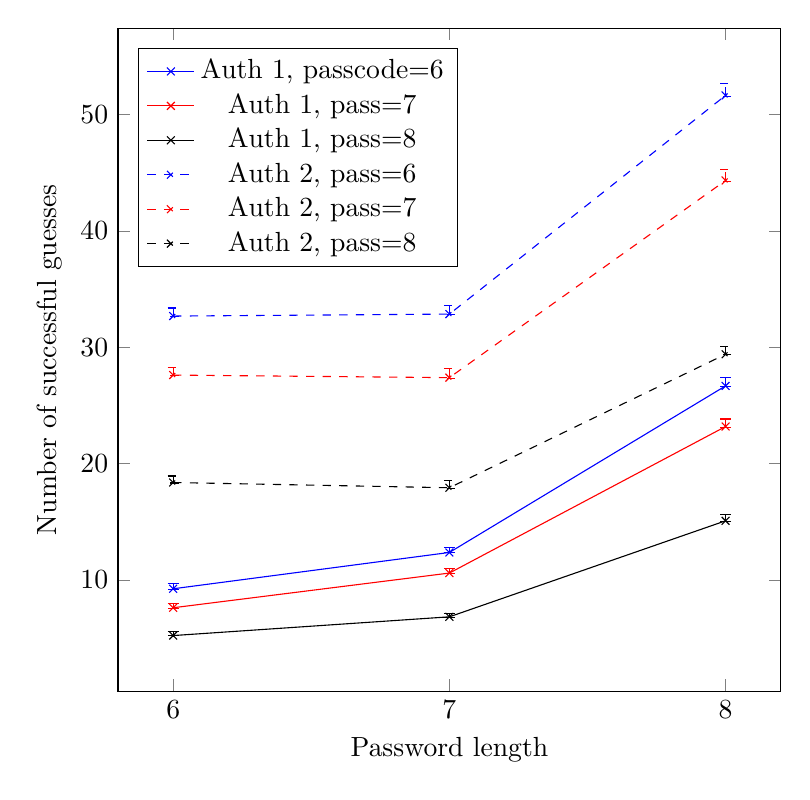
\begin{tikzpicture}
	    \begin{axis}[
	    	height=10cm,
	    	width=10cm,
	    	xtick={6,7,8},
	        xlabel=Password length,
	        ylabel=Number of successful guesses,
	        legend pos=north west
	    ]
	    \addplot[
	        mark=x,
	        blue,
	        error bars/.cd, y dir=both, y explicit,
	    ] plot coordinates {
	        (6,9.25)   -=(0,0.033) += (0,0.438)
	        (7,12.37)  -=(0,0.034) += (0,0.450)
	        (8,26.68)  -=(0,0.058) += (0,0.759)
	    };
	    \addlegendentry{Auth 1, passcode=6}

	    \addplot[
	        mark=x,
	        red,
	        error bars/.cd, y dir=both, y explicit,
	    ] plot coordinates {
	        (6,7.62)  -= (0,0.030) += (0,0.398)
	        (7,10.60) -= (0,0.030) += (0,0.397)
	        (8,23.19) -= (0,0.049) += (0,0.645)
	    };
	    \addlegendentry{Auth 1, pass=7}    

	    \addplot[
	        mark=x,
	        error bars/.cd, y dir=both, y explicit,
	    ] plot coordinates {
	        (6,5.23)  -= (0,0.025) += (0,0.329)
	        (7,6.84)  -= (0,0.024) += (0,0.319)
	        (8,15.09) -= (0,0.039) += (0,0.504)
	    };
	    \addlegendentry{Auth 1, pass=8}

	    \addplot[
	        mark=x,
	        blue,
	        dashed,
	        error bars/.cd, y dir=both, y explicit,
	    ] plot coordinates {
	        (6,32.68)  -=(0,0.053) += (0,0.695)
	        (7,32.85)  -=(0,0.058) += (0,0.753)
	        (8,51.64)  -=(0,0.078) += (0,1.026)
	    };
	    \addlegendentry{Auth 2, pass=6}

	    \addplot[
	        mark=x,
	        red,
	        dashed,
	        error bars/.cd, y dir=both, y explicit,
	    ] plot coordinates {
	        (6,27.61) -= (0,0.053) += (0,0.690)
	        (7,27.39) -= (0,0.057) += (0,0.749)
	        (8,44.33) -= (0,0.070) += (0,0.921)
	    };
	    \addlegendentry{Auth 2, pass=7}    

	    \addplot[
	        mark=x,
	        dashed,
	        error bars/.cd, y dir=both, y explicit,
	    ] plot coordinates {
	        (6,18.38)  -= (0,0.043) += (0,0.559)
	        (7,17.93)  -= (0,0.046) += (0,0.599)
	        (8,29.40)  -= (0,0.049) += (0,0.645)
	    };
	    \addlegendentry{Auth 2, pass=8}

	    \end{axis}
	\end{tikzpicture}
	\caption{Mean number of successful guesses from ($50 \times 10^6 $) attempts using varying passcode length}
	\label{fig:approach_comparison}
\end{figure}

\begin{figure}
	\begin{tikzpicture}
	    \begin{axis}[ybar, xtick = {6,7,8}, xlabel = Minimum password length, ylabel = Number of valid account passwords in \cite{rockyoupasswords}]
		\addplot table [
		        col sep=comma,
		        x=pass_size,
		        y=num_pass,
		    ] {data/password_count.csv};
	    \end{axis}	    
	    \begin{axis}[
	    	axis y line*=right,
    		axis x line=none, 
    		ylabel = Number of valid attack passwords out of 500]
		\addplot table [
		        col sep=comma,
		        x=pass_size,
		        y=guess_pass,
		    ] {data/password_count.csv};
	    \end{axis}
	\end{tikzpicture}
	\caption{Count of valid passwords in \cite{rockyoupasswords} for each password policy}
	\label{fig:passwords_length}
\end{figure}


\subsection{Counter-measures}




\clearpage
\bibliographystyle{IEEEtranSN}
\bibliography{references}
\clearpage
\begin{appendices}

	\section{Main.py}\label{app:main}
	\lstinputlisting[language=Python]{../main.py}

	\section{Additional statistics}\label{app:extra_stats}
	\subsection{Individual statistics}
	\begin{table}[]
		\centering
		\begin{tabular}{|l|l|l|l|l|l|l|l|}
		\hline
		& & \multicolumn{6}{l|}{\textbf{Auth system and password length}} \\ \hline
		\textbf{Mean} & \textbf{Password len} & \textbf{Auth1, 6} & \textbf{Auth1, 7} & \textbf{Auth1, 8} & \textbf{Auth2, 6} & \textbf{Auth2, 7} & \textbf{Auth2, 8} \\ \hline
		 & 6 & 9.25 & 7.62 & 5.23 & 32.68 & 27.61 & 18.38 \\ \hline
		 & 7 & 12.37 & 10.60 & 6.84 & 32.85 & 27.39 & 17.93 \\ \hline
		 & 8 & 26.68 & 23.19 & 15.09 & 51.64 & 44.33 & 29.40 \\ \hline
		\textbf{Median} &  &  &  &  &  &  &  \\ \hline
		 & 6 & 9.00 & 7.00 & 5.00 & 33.00 & 28.00 & 18.00 \\ \hline
		 & 7 & 12.00 & 10.50 & 6.50 & 33.00 & 28.00 & 18.00 \\ \hline
		 & 8 & 27.00 & 23.00 & 15.00 & 52.00 & 44.50 & 29.00 \\ \hline
		\textbf{STD} &  &  &  &  &  &  &  \\ \hline
		 & 6 & 3.26 & 2.96 & 2.45 & 5.17 & 5.14 & 4.16 \\ \hline
		 & 7 & 3.35 & 2.95 & 2.38 & 5.61 & 5.58 & 4.46 \\ \hline
		 & 8 & 5.65 & 4.80 & 3.75 & 7.64 & 6.86 & 4.80 \\ \hline
		\textbf{Min} &  &  &  &  &  &  &  \\ \hline
		 & 6 & 2.00 & 2.00 & 1.00 & 21.00 & 16.00 & 9.00 \\ \hline
		 & 7 & 5.00 & 4.00 & 2.00 & 21.00 & 10.00 & 6.00 \\ \hline
		 & 8 & 12.00 & 11.00 & 3.00 & 32.00 & 27.00 & 20.00 \\ \hline
		\textbf{Max} &  &  &  &  &  &  &  \\ \hline
		 & 6 & 18.00 & 15.00 & 14.00 & 46.00 & 43.00 & 29.00 \\ \hline
		 & 7 & 21.00 & 20.00 & 13.00 & 48.00 & 43.00 & 31.00 \\ \hline
		 & 8 & 43.00 & 38.00 & 24.00 & 75.00 & 64.00 & 44.00 \\ \hline
		\textbf{0.1 confidence} &  &  &  &  &  &  &  \\ \hline
		 & 6 & 0.033 & 0.030 & 0.025 & 0.053 & 0.053 & 0.043 \\ \hline
		 & 7 & 0.034 & 0.030 & 0.024 & 0.058 & 0.057 & 0.046 \\ \hline
		 & 8 & 0.058 & 0.049 & 0.039 & 0.078 & 0.070 & 0.049 \\ \hline
		\textbf{0.9 confidence} &  &  &  &  &  &  &  \\ \hline
		 & 6 & 0.438 & 0.398 & 0.329 & 0.695 & 0.690 & 0.559 \\ \hline
		 & 7 & 0.450 & 0.397 & 0.319 & 0.753 & 0.749 & 0.599 \\ \hline
		 & 8 & 0.759 & 0.645 & 0.504 & 1.026 & 0.921 & 0.645 \\ \hline
		\end{tabular}
		\caption{Individual statistics for each authentication system and password/passcode length combination}
	\end{table}
  	\clearpage

  	\subsection{Data significance}
  	\label{app:significant_stats}
  	The following table details the results of statistical tests between each authentication system using equivalent password/passcode length policies.
  	\begin{table}[h]
	\centering
	\begin{tabular}{|l|l|l|l|l|}
	\hline
	Password/Passcode length & Auth 1 median & Auth 2 median & Mann whitney Z-score & p value \\ \hline
	6,6 & 9 & 33 & -14.974 & p\textless0.01 \\ \hline
	6,7 & 7 & 27.5 & -14.974 & p\textless0.01 \\ \hline
	6,8 & 5 & 18 & -15.100 & p\textless0.01 \\ \hline
	7,6 & 12 & 33 & -14.974 & p\textless0.01 \\ \hline
	7,7 & 10.5 & 28 & -14.793 & p\textless0.01 \\ \hline
	7,8 & 6.5 & 18 & -14.596 & p\textless0.01 \\ \hline
	8,6 & 27 & 52 & -14.898 & p\textless0.01 \\ \hline
	8,7 & 23 & 44.5 & -14.801 & p\textless0.01 \\ \hline
	8,8 & 15 & 29 & -14.794 & p\textless0.01 \\ \hline
	\end{tabular}
	\caption{Statistical tests between authentication systems for equivalent password/passcode length}
	\label{tab:significance}
	\end{table}
\end{appendices}
\clearpage
\end{document}
